\documentclass[aspectratio=169]{beamer}
\usetheme{Madrid}
\usepackage[utf8]{inputenc}
\usepackage{graphicx}
\usepackage{hyperref}
\usepackage{listings}
\usepackage{amssymb}
\usepackage{xcolor}
\usepackage{tikz}
\usetikzlibrary{shapes.geometric, arrows, calc}
\hypersetup{colorlinks=true, linkcolor=purpleprimary, urlcolor=orangeprimary}

% =============================================================================
% DopamiNah Brand Colors
% =============================================================================
\definecolor{purpleprimary}{HTML}{8B5CF6}
\definecolor{purpledark}{HTML}{6D28D9}
\definecolor{purplelight}{HTML}{DDD6FE}
\definecolor{orangeprimary}{HTML}{FA832B}
\definecolor{bglight}{HTML}{F8FAFC}
\definecolor{textprimary}{HTML}{0F172A}
\definecolor{textsecondary}{HTML}{64748B}
\definecolor{bgdark}{HTML}{1C1B1F}
\definecolor{surfacedark}{HTML}{2B2930}
\definecolor{braindeeppurple}{HTML}{8D459F}
\definecolor{brainmuted}{HTML}{CAAFD8}
\definecolor{brainlight}{HTML}{D9C8E8}

% =============================================================================
% Beamer Theme Colors — DopamiNah Purple & Orange
% =============================================================================
\setbeamercolor{structure}{fg=purpleprimary}
\setbeamercolor{palette primary}{bg=purpleprimary, fg=white}
\setbeamercolor{palette secondary}{bg=purpledark, fg=white}
\setbeamercolor{palette tertiary}{bg=orangeprimary, fg=white}
\setbeamercolor{titlelike}{parent=palette primary}
\setbeamercolor{block title}{bg=purpleprimary, fg=white}
\setbeamercolor{block body}{bg=purplelight!20, fg=textprimary}
\setbeamercolor{section in head/foot}{bg=purpleprimary!85, fg=white}
\setbeamercolor{background canvas}{bg=bglight}
\setbeamercolor{normal text}{fg=textprimary}
\setbeamercolor{alerted text}{fg=orangeprimary}
\setbeamercolor{itemize item}{fg=purpleprimary}
\setbeamercolor{itemize subitem}{fg=orangeprimary}
\setbeamercolor{enumerate item}{fg=purpleprimary}
\setbeamercolor{enumerate subitem}{fg=orangeprimary}

% Title page styling
\setbeamertemplate{title page}{%
  \begin{tikzpicture}[remember picture, overlay]
    \fill[purpleprimary] (current page.north west) rectangle (current page.south east);
    \node[anchor=center] at (current page.center) {
      \begin{minipage}{0.85\textwidth}
        \centering
        \brainicon[2cm] \\[0.4cm]
        {\usebeamerfont{title}\color{white}\inserttitle\par}
        \vspace{0.3cm}
        {\usebeamerfont{subtitle}\color{purplelight}\insertsubtitle\par}
        \vspace{0.5cm}
        {\usebeamerfont{author}\color{white}\insertauthor\par}
        \vspace{0.2cm}
        {\usebeamerfont{institute}\color{purplelight!80}\insertinstitute\par}
        \vspace{0.1cm}
        {\usebeamerfont{date}\color{purplelight!80}\insertdate\par}
      \end{minipage}
    };
  \end{tikzpicture}%
}

% Footer
\setbeamercolor{author in head/foot}{bg=purpleprimary, fg=white}
\setbeamercolor{title in head/foot}{bg=purpledark, fg=purplelight}
\setbeamercolor{date in head/foot}{bg=purpleprimary, fg=white}
\setbeamercolor{page number in head/foot}{bg=purpleprimary, fg=white}

% =============================================================================
% Brain Icon (from project favicon)
% =============================================================================
\newcommand{\brainicon}[1][2cm]{%
  \includegraphics[width=#1]{../screenshots/dopaminah-icon.png}%
}

% Phone mockup placeholder
\newcommand{\phonemockup}[1][5.5cm]{%
  \begin{tikzpicture}[x=#1, y=#1, scale=0.025]
    \draw[purpleprimary, very thick, rounded corners=1.5] (0,0) rectangle (8,16);
    \draw[purpleprimary!30, rounded corners=0.8] (0.6,1) rectangle (7.4,15);
    \fill[purpleprimary!10] (0.6,1) rectangle (7.4,15);
    \draw[purpleprimary!50, rounded corners=0.3] (3.2,15.2) rectangle (4.8,15.8);
    \node[purpleprimary!60] at (4,14.2) {\tiny\textbf{DopamiNah}};
    \draw[purpleprimary!40] (0.8,13.5) -- (7.2,13.5);
    \node[purpleprimary!40] at (4,12) {\tiny [Pantalla]};
  \end{tikzpicture}%
}

% Browser mockup placeholder
\newcommand{\browsermockup}[1][6cm]{%
  \begin{tikzpicture}[x=#1, y=#1, scale=0.022]
    \draw[purpleprimary, very thick, rounded corners=0.6] (0,0) rectangle (14,10);
    \fill[purpleprimary!8] (0,0) rectangle (14,10);
    \fill[purpleprimary!70, rounded corners=0.3] (0.5,9) rectangle (1.5,9.6);
    \fill[orangeprimary!60, rounded corners=0.2] (0.7,9.05) rectangle (1,9.3);
    \fill[orangeprimary!60, rounded corners=0.2] (1.05,9.05) rectangle (1.35,9.3);
    \draw[purpleprimary!40, rounded corners=0.2] (2,9.1) rectangle (10,9.5);
    \node[purpleprimary!50] at (6,9.3) {\tiny\texttt{dominio.com}};
    \draw[purpleprimary!30] (0.5,8.5) -- (13.5,8.5);
    \node[purpleprimary!40] at (7,7) {\tiny [P\'agina Web]};
  \end{tikzpicture}%
}

\title[DopamiNah]{DopamiNah: Control de Adicción Digital}
\subtitle{Microproyecto --- Kotlin Multiplatform}
\author{Fredy, Julián}
\institute{Universidad del Cauca}
\date{\today}

% Title page with brain icon
\titlegraphic{\brainicon[1.8cm]}

\begin{document}

\begin{frame}
  \titlepage
\end{frame}

%----------------------------------------------------------
\section{Descripción de la App}
\begin{frame}{¿Qué es DopamiNah?}
  \begin{columns}[T]
    \begin{column}{0.58\textwidth}
      \textbf{DopamiNah} es un sistema multiplataforma para reducir la adicción digital
      mediante límites de tiempo en aplicaciones (Android) y sitios web (Web).

      \vspace{0.3cm}
      \textbf{Características:}
      \begin{itemize}
        \item Monitoreo de uso en tiempo real.
        \item Metas personalizables con límites diarios.
        \item Gamificación (rachas, insignias, niveles).
        \item Navegador Focus con bloqueo restrictivo.
        \item Sincronización con extensión de navegador.
      \end{itemize}

      \vspace{0.15cm}
      \centering
      \textit{``Toma el control de tu tiempo digital.''}
    \end{column}
    \begin{column}{0.42\textwidth}
      \centering
      \phonemockup[4.5cm]
    \end{column}
  \end{columns}
\end{frame}

\begin{frame}{Restricción en Apps Móviles (Android)}
  \textbf{Monitoreo de uso de aplicaciones:}
  \begin{itemize}
    \item Uso de \texttt{UsageStatsManager} para consultar el tiempo de uso por app.
    \item Metas asignadas a paquetes específicos (\texttt{com.example.app}).
    \item Bloqueo automático al alcanzar el límite diario mediante \texttt{App Blocker}.
  \end{itemize}

  \vspace{0.2cm}
  \textbf{Flujo de restricción:}
  \begin{enumerate}
    \item El usuario define un límite diario para una app (ej. 30 min para Instagram).
    \item El \texttt{DeviceUsageRepository} monitorea el tiempo acumulado.
    \item Al superar el límite, el App Blocker intercepta la apertura.
    \item Se muestra una notificación o pantalla de bloqueo.
  \end{enumerate}

  \vspace{0.2cm}
  \textbf{Tecnologías:} \texttt{UsageStatsManager}, \texttt{PackageManager},
  \texttt{Service} en segundo plano.
\end{frame}

\begin{frame}{Restricción en Sitios Web (Web)}
  \textbf{Monitoreo de navegación por dominio:}
  \begin{itemize}
    \item Control de tiempo por dominio (\texttt{youtube.com}, \texttt{twitter.com}).
    \item Integración con extensión de navegador (Chrome/Edge MV3).
    \item Bloqueo mediante \texttt{Declarative Net Request (DNR)} rules.
    \item Navegador Focus embebido con WebView sandbox.
  \end{itemize}

  \vspace{0.2cm}
  \textbf{Flujo de restricción:}
  \begin{enumerate}
    \item El usuario configura un límite para un dominio (ej. 20 min para YouTube).
    \item La extensión monitorea el tiempo activo mediante \texttt{chrome.webNavigation}.
    \item Al agotar el tiempo, se activan reglas DNR de redirección.
    \item El usuario ve una página de bloqueo con estadísticas del día.
  \end{enumerate}

  \vspace{0.2cm}
  \textbf{Tecnologías:} Extensión Manifest V3, \texttt{webNavigation},
  \texttt{declarativeNetRequest}, WebView compartido.
\end{frame}

%----------------------------------------------------------
\section{Créditos}
\begin{frame}{Créditos del Proyecto}
  \textbf{Repositorio:} \href{https://github.com/Crownyny/DopamiNah}{github.com/Crownyny/DopamiNah} \\
  Universidad del Cauca.

  \vspace{0.5cm}
  \begin{columns}[T]
    \begin{column}{0.45\textwidth}
      \textbf{Desarrolladores:}
      \begin{itemize}
        \item \textbf{Fredy} — Android / Shared Module
        \item \textbf{Julián} — Android / UI / Testing
      \end{itemize}
    \end{column}
    \begin{column}{0.55\textwidth}
      \textbf{Rama:}
      \begin{itemize}
        \item \texttt{dev-kmp} — Desarrollo principal del proyecto KMP.
      \end{itemize}
    \end{column}
  \end{columns}

  \vspace{0.4cm}
  \textbf{Tecnologías:} Kotlin Multiplatform, Compose Multiplatform, Voyager, Koin,
  Multiplatform-Settings, Ktor, Coil.
\end{frame}

%----------------------------------------------------------
\section{Objetivos y Requisitos}
\begin{frame}{Requisitos Cubiertos}
  \begin{enumerate}
    \item[\checkmark] \textbf{Despliegue en 2+ plataformas} — Android y Web (JS/Wasm).
    \item[\checkmark] \textbf{5+ pantallas} — Android: 6 (Onboarding, Dashboard, Stats, Goals, Achievements, Settings). Web: 4 (Goals, Navegaci\'on, Achievements, Settings).
    \item[\checkmark] \textbf{Persistencia de datos} — \texttt{multiplatform-settings} (SharedPreferences/NSUserDefaults), próximamente SQLDelight.
    \item[\checkmark] \textbf{Navegación en capa compartida} — Voyager + Tab Navigation gestionados en \texttt{commonMain}.
    \item[\checkmark] \textbf{Repositorio GIT público} con ramas por estudiante y commits visibles.
    \item[\checkmark] \textbf{Vista de créditos} con descripción de la app y nombres de los estudiantes.
  \end{enumerate}
\end{frame}

%----------------------------------------------------------
\section{Arquitectura}
\begin{frame}{Arquitectura del Proyecto}
  \centering
  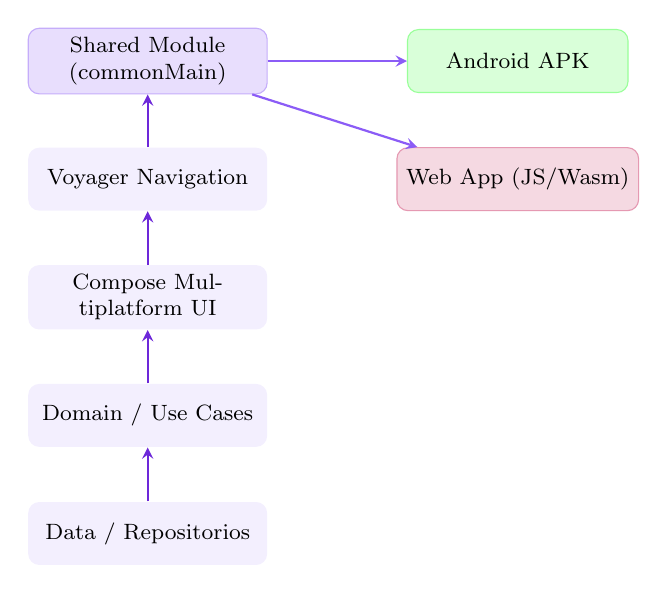
\begin{tikzpicture}[
    node distance=1.2cm,
    box/.style={rectangle, minimum width=2.8cm, minimum height=0.8cm, rounded corners, text centered, font=\footnotesize},
    arrow/.style={thick,->,>=stealth}
  ]

    % Shared Module — purple gradient
    \node[box, fill=purpleprimary!20, text width=2.8cm, draw=purpleprimary!50] (shared) {Shared Module (commonMain)};
    \node[box, fill=purpleprimary!10, below of=shared, yshift=-0.3cm, text width=2.8cm] (nav) {Voyager Navigation};
    \node[box, fill=purpleprimary!10, below of=nav, yshift=-0.3cm, text width=2.8cm] (ui) {Compose Multiplatform UI};
    \node[box, fill=purpleprimary!10, below of=ui, yshift=-0.3cm, text width=2.8cm] (domain) {Domain / Use Cases};
    \node[box, fill=purpleprimary!10, below of=domain, yshift=-0.3cm, text width=2.8cm] (data) {Data / Repositorios};

    % Platforms — Android green, Web purple
    \node[box, fill=green!15, right of=shared, xshift=3.5cm, draw=green!40] (android) {Android APK};
    \node[box, fill=purple!15, below of=android, yshift=-0.3cm, draw=purple!40] (web) {Web App (JS/Wasm)};

    \draw[arrow, purpleprimary] (shared) -- (android);
    \draw[arrow, purpleprimary] (shared) -- (web);
    \draw[arrow, purpledark] (nav) -- (shared);
    \draw[arrow, purpledark] (ui) -- (nav);
    \draw[arrow, purpledark] (domain) -- (ui);
    \draw[arrow, purpledark] (data) -- (domain);
  \end{tikzpicture}
\end{frame}

%----------------------------------------------------------
\section{Pantallas}
\begin{frame}{Pantallas por Plataforma}
  \begin{columns}[T]
    \begin{column}{0.45\textwidth}
      \centering\textbf{\textcolor{purpleprimary}{Android (5 pantallas)}}\\[0.2cm]
      \begin{itemize}
        \item \textbf{Onboarding} --- Permisos de uso (1 vez).
        \item \textbf{Dashboard (Inicio)} --- Resumen diario y apps m\'as usadas.
        \item \textbf{Stats} --- Gr\'aficos de uso por app.
        \item \textbf{Goals (Metas)} --- L\'imites por aplicaci\'on.
        \item \textbf{Achievements (Logros)} --- Insignias y rachas.
        \item \textbf{Settings (Ajustes)} --- Tema, sincronizaci\'on.
      \end{itemize}
      Oculta la pesta\~na \texttt{Navegaci\'on}.
    \end{column}
    \begin{column}{0.45\textwidth}
      \centering\textbf{\textcolor{orangeprimary}{Web (4 pantallas)}}\\[0.2cm]
      \begin{itemize}
        \item \textbf{Goals (Metas)} --- L\'imites por dominio web.
        \item \textbf{Navegaci\'on} --- Estad\'isticas de navegaci\'on por dominio.
        \item \textbf{Achievements (Logros)} --- Insignias y rachas.
        \item \textbf{Settings (Ajustes)} --- Tema, sincronizaci\'on.
      \end{itemize}
      Oculta \texttt{Dashboard} y \texttt{Stats} (no aplican en Web).
    \end{column}
  \end{columns}

  \vspace{0.3cm}
  \centering
  \textbf{Navegaci\'on compartida:} \texttt{commonMain} con Voyager + tabs condicionales por plataforma.
\end{frame}

%----------------------------------------------------------
\section{Persistencia}
\begin{frame}{Persistencia de Datos}
  \textbf{Mecanismo actual:} \texttt{multiplatform-settings} (librería \texttt{russhwolf})

  \vspace{0.3cm}
  \begin{itemize}
    \item \textbf{Android:} \texttt{SharedPreferences}
    \item \textbf{Web:} \texttt{multiplatform-settings} (JS)
  \end{itemize}

  \vspace{0.3cm}
  \textbf{Datos persistentes:}
  \begin{itemize}
    \item[] Metas y límites de tiempo por aplicación/dominio.
    \item[] Estadísticas de uso diario y horario.
    \item[] Estado de gamificación (rachas, puntos, nivel, insignias).
    \item[] Preferencias de tema (oscuro/claro) y suscripción premium.
    \item[] Estado de sincronización con la extensión de navegador.
  \end{itemize}

  \vspace{0.2cm}
  \textbf{Próximamente:} Migración a \texttt{SQLDelight} (v2.0.2) como base de datos relacional.
\end{frame}

%----------------------------------------------------------
\section{Navegación}
\begin{frame}{Navegación en Capa Compartida (KMP)}
  \textbf{Librería:} \texttt{Voyager 1.1.0-beta03}

  \vspace{0.3cm}
  \begin{itemize}
    \item La navegación se define en \texttt{commonMain} con un \texttt{TabNavigator}.
    \item Cada pantalla es un \texttt{Screen} de Voyager con su propio \texttt{ViewModel}.
    \item El \texttt{AppState} centralizado controla el flujo (Onboarding $\rightarrow$ App).
    \item Las plataformas solo proveen el contenedor raíz:
      \begin{itemize}
        \item \textbf{Android:} \texttt{setContent \{ App() \}}
        \item \textbf{Web:} \texttt{ComposeWidget()} montado en el DOM.
      \end{itemize}
  \end{itemize}

  \vspace{0.3cm}
  \textbf{Ejemplo de pantallas (sealed class):}
  \begin{center}
  \texttt{\tiny
  sealed class Screen(val route: String, val title: String) \{\\
  \ \ \ \ object Dashboard : Screen("dashboard", "Inicio")\\
  \ \ \ \ object Stats : Screen("stats", "Stats")\\
  \ \ \ \ object Goals : Screen("goals", "Metas")\\
  \ \ \ \ object Achievements : Screen("achievements", "Logros")\\
  \ \ \ \ object Settings : Screen("settings", "Ajustes")\\
  \ \ \ \ object Onboarding : Screen("onboarding", "Permisos")\\
  \}
  }
  \end{center}
\end{frame}

%----------------------------------------------------------
\section{GIT}
\begin{frame}{Repositorio GIT y Ramas}
  \begin{center}
\href{https://github.com/Crownyny/DopamiNah}{github.com/Crownyny/DopamiNah}
  \end{center}
  \vspace{-0.3cm}

  \vspace{0.3cm}
  \textbf{Rama:}
  \begin{itemize}
    \item \texttt{dev-kmp} — Desarrollo principal del proyecto KMP.
  \end{itemize}

  \vspace{0.3cm}
  \textbf{Commits destacados:}
  \begin{itemize}
    \small
    \item \texttt{4d8ade1} — Initial KMP project scaffold
    \item \texttt{7233ba5} — Full KMP migration plan phases 1-4 and 6
    \item \texttt{89ab903} — Full UI screens matching Android native branch
    \item \texttt{c405487} — Full statistics screen and data integration
    \item \texttt{6e06cb7} — Goals management with real-time usage tracking
    \item \texttt{cbf0def} — Comprehensive UI updates (Settings + Achievements)
    \item \texttt{97fdd75} — Status bar color fixed / goals section fixed
    \item \texttt{39f5121} — Android: Add App Blocker
  \end{itemize}
\end{frame}

%----------------------------------------------------------
\section{Reflexión}
\begin{frame}{Reflexión: Multiplataforma vs Nativo}
  \textbf{Desarrollo Nativo (Android/iOS)}:
  \begin{itemize}
    \item Acceso completo a APIs del sistema (UsageStatsManager, NotificationManager).
    \item Mejor rendimiento en UI compleja y animaciones.
    \item Código duplicado: lógica de negocio separada por plataforma.
    \item Mayor tiempo de desarrollo para mantener dos o más codebases.
  \end{itemize}

  \vspace{0.2cm}
  \textbf{Kotlin Multiplatform --- Ventajas}:
  \begin{itemize}
    \item Una sola base de código para lógica de negocio, navegación y UI con Compose Multiplatform.
    \item Reducción significativa de código duplicado entre plataformas.
    \item Sincronización entre plataformas más sencilla (mismos repositorios, mismos ViewModels).
  \end{itemize}
\end{frame}

\begin{frame}{Reflexión: Desafíos}
  \textbf{Kotlin Multiplatform --- Desafíos}:
  \begin{itemize}
    \item Limitaciones en APIs específicas (ej. monitoreo de uso requiere \texttt{expect/actual}).
    \item Madurez relativa de Compose Multiplatform frente a SwiftUI / Jetpack Compose nativo.
    \item Curva de aprendizaje inicial para configurar correctamente los targets multiplataforma.
  \end{itemize}
\end{frame}

\begin{frame}{Reflexión: Conclusión}
  \textbf{Conclusión:}

  \medskip
  KMP es ideal para aplicaciones con lógica compartida compleja que deben ejecutarse en
  múltiples plataformas. Para características que dependen fuertemente del hardware o del
  sistema operativo nativo, el enfoque \texttt{expect/actual} permite mantener la
  reutilización del código sin sacrificar la funcionalidad específica de cada plataforma.

  \medskip
  La experiencia con DopamiNah demostró que la productividad aumenta significativamente al
  compartir la capa de navegación, los ViewModels y la UI en Compose Multiplatform,
  reduciendo el tiempo de desarrollo a aproximadamente la mitad en comparación con
  mantener dos proyectos nativos separados.
\end{frame}

%----------------------------------------------------------
\section{Capturas}
\begin{frame}{Capturas --- Android (1/2)}
  \centering
  \textbf{Dashboard y Stats}
  \vspace{0.3cm}

  \begin{columns}[T]
    \begin{column}{0.45\textwidth}
      \centering
      \fcolorbox{purpleprimary}{bglight}{\parbox{0.85\textwidth}{\centering\vspace{3cm}
        \textbf{\textcolor{purpleprimary}{[Dashboard]}}\vspace{3cm}
      }}
      \par
      \tiny{Dashboard --- Resumen diario}
    \end{column}
    \begin{column}{0.45\textwidth}
      \centering
      \fcolorbox{purpleprimary}{bglight}{\parbox{0.85\textwidth}{\centering\vspace{3cm}
        \textbf{\textcolor{purpleprimary}{[Stats]}}\vspace{3cm}
      }}
      \par
      \tiny{Stats --- Gr\'aficos de uso}
    \end{column}
  \end{columns}
\end{frame}

\begin{frame}{Capturas --- Android (2/2)}
  \centering
  \textbf{Goals (Metas) y Achievements (Logros)}
  \vspace{0.3cm}

  \begin{columns}[T]
    \begin{column}{0.45\textwidth}
      \centering
      \fcolorbox{purpleprimary}{bglight}{\parbox{0.85\textwidth}{\centering\vspace{3cm}
        \textbf{\textcolor{purpleprimary}{[Metas]}}\vspace{3cm}
      }}
      \par
      \tiny{Metas --- L\'imites por app}
    \end{column}
    \begin{column}{0.45\textwidth}
      \centering
      \fcolorbox{purpleprimary}{bglight}{\parbox{0.85\textwidth}{\centering\vspace{3cm}
        \textbf{\textcolor{purpleprimary}{[Logros]}}\vspace{3cm}
      }}
      \par
      \tiny{Logros --- Gamificaci\'on}
    \end{column}
  \end{columns}
\end{frame}

\begin{frame}{Capturas --- Web (1/2)}
  \centering
  \textbf{Goals (Metas por dominio) y Navegaci\'on}
  \vspace{0.3cm}

  \begin{columns}[T]
    \begin{column}{0.45\textwidth}
      \centering
      \fcolorbox{orangeprimary}{bglight}{\parbox{0.85\textwidth}{\centering\vspace{3cm}
        \textbf{\textcolor{orangeprimary}{[Metas Web]}}\vspace{3cm}
      }}
      \par
      \tiny{Metas --- L\'imites por dominio}
    \end{column}
    \begin{column}{0.45\textwidth}
      \centering
      \fcolorbox{orangeprimary}{bglight}{\parbox{0.85\textwidth}{\centering\vspace{3cm}
        \textbf{\textcolor{orangeprimary}{[Navegaci\'on]}}\vspace{3cm}
      }}
      \par
      \tiny{Navegaci\'on --- Stats de navegaci\'on}
    \end{column}
  \end{columns}
\end{frame}

\begin{frame}{Capturas --- Web (2/2)}
  \centering
  \textbf{Achievements (Logros) y Settings (Ajustes)}
  \vspace{0.3cm}

  \begin{columns}[T]
    \begin{column}{0.45\textwidth}
      \centering
      \fcolorbox{orangeprimary}{bglight}{\parbox{0.85\textwidth}{\centering\vspace{3cm}
        \textbf{\textcolor{orangeprimary}{[Logros]}}\vspace{3cm}
      }}
      \par
      \tiny{Logros --- Gamificaci\'on}
    \end{column}
    \begin{column}{0.45\textwidth}
      \centering
      \fcolorbox{orangeprimary}{bglight}{\parbox{0.85\textwidth}{\centering\vspace{3cm}
        \textbf{\textcolor{orangeprimary}{[Ajustes]}}\vspace{3cm}
      }}
      \par
      \tiny{Ajustes --- Tema y sincronizaci\'on}
    \end{column}
  \end{columns}

  \vspace{0.3cm}
  \textit{Reemplace estos marcadores con capturas reales en \texttt{docs/screenshots/}.}
\end{frame}

%----------------------------------------------------------
\section*{}
\begin{frame}
  \centering
  \brainicon[2.5cm] \\[0.3cm]
  \Large{\textbf{\textcolor{purpleprimary}{Gracias}}} \\[0.5cm]
  \normalsize
  \texttt{github.com/Crownyny/DopamiNah} \\[0.3cm]
  \small
  \textcolor{textsecondary}{DopamiNah --- ``Toma el control de tu tiempo digital''} \\[0.3cm]
  Universidad del Cauca, 2025/2026
\end{frame}

\end{document}
